\section{Použité technológie a prostredie}
\subsection{OpenCV}
\acrfull{OpenCV} bola pôvodne vydávaná firmou Intel, neskôr výskumným centrom Willow Garage, ktoré vyvíja open source softvér pre aplikácie na poli robotiky. Podporuje frameworky TensorFlow, Torch/PyTorch, Caffe. Knižnica je vydávaná pod BSD licenciou, čo umožňuje jej komerčné používanie. Táto knižnica obsahuje množstvo nástrojov a algoritmov na detegovanie gest, identifikáciu objektov, segmentáciu a rozpoznávanie, spájanie obrazov, sledovanie pohybu, taktiež je vhodná pre implementáciu rozšírenej reality a strojového učenia. OpenCV je podporované v jazykoch C++, Python, Java, C a Matlab. Vývoj je umožnený na operačných systémov Windows, Android, Linux a Mac. \cite{c4}


\subsection{FFmpeg}
Táto knižnica je voľný softvérový projekt určený na manipulovanie (kódovanie, dekódovanie, multiplexovanie, prehrávanie a streamovanie) s multimediálnymi súbormi. Má voľnú licenciu GNU (General Public License). Výhodou práce s knižnicou FFmpeg je jej rýchlosť a kvalita výstupných dát. Knižnicu využíva aj OpenCV pre spracovanie a distribuovanie obrazovej sekvencie. Obsahuje nástroje na zmenu kvality videa, strihanie, čo napomáha pri kontextovej analýze obrazu.\cite{c9}

\subsection{Python}
Programovací jazyk Python je interpretovaný vysokoúrovňový jazyk, vytvorený v roku 1991. Jeho využitie je široké, od vývoja webových aplikácii, backendu, frontendu cez vedecké a numerické výpočty, tvorbu grafických rozhraní, vývoj softvéru, výučbu a tvorbu biznis aplikácií. V súčasnosti má širokú podporu u programátorov, čo sa odráža aj na prehľadnom zdokumentovaní. Je to open source softvér s množstvom štandardných knižníc, ktoré majú široké využitie v automatizácii, multimédiách, spracovaní obrazu, textu a ďalších sférach IT.\cite{c6}
\subsection{Scikit a Numpy}

\subsubsection{Scikit}
Scikit-learn je knižnica s otvoreným zdrojovým kódom pre strojové učenie pre programovací jazyk Python. Scikit je napísaný v jazyku Python s niektorými algoritmami písanými v Cythone pre zvýšenie výkonu tejto knižnice. Obsahuje rôzne klasifikačné, regresné a zhlukovacie algoritmy, taktiež algoritmy na modelovanie dát (krížová validácia, výber príznakov, clustering a iné). Je navrhnutá na spoluprácu s numerickou knižnicou NumPy a vedeckou knižnicou SciPy. \cite{c5}

\subsubsection{NumPy}
NumPy je rozšírenie do Pythonu, ktoré nám umožňuje rýchle a efektívne vykonávanie operácií nad poľami homogénnych dát. NumPy pole je multidimenzionálne pole objektov ktoré majú všetky rovnaký typ. V pamäti sa nachádza ako objekt, ktorý smeruje na blok pamäte, ktorý drží informáciu o type údajov v pamäti, počet dimenzií pamäte, veľkosť každej dimenzie a taktiež aj vzdialenosti medzi jednotlivými prvkami pozdĺž každej z osí. Narozdiel od klasického zoznamu, ktorý je implementovaný ako zoznam smerníkov je prehľadávanie NumPy poľa rýchlejšie. klasický zoznam potrebuje na iteráciu poľa prístup cez dva smerníky, čo predĺžuje čas prehľadávania.\cite{c8}


\section{Princípy riešenia}
V prvej časti tejto práce si predstavíme  metódy, ktoré sme zvažovali pri riešení nášho problému. Takisto si zhrnieme aké databázy pohybov máme k dispozícii pre potreby tejto práce, typy databáz, dĺžky jednotlivých videí, vlastnosti a aké druhy aktivít sa v týchto videách nachádzajú. Taktiež je potrebné predstaviť metodológiu spracovania údajov pre zachytenie vhodných vlastností videa na rozpoznanie. Na obrázku \ref{UML1} je znázornená predstava riešenia problému detekcie a rozpoznávania pohybu. Základom je načítanie videí, následne ich predspracovanie na extrakciu príznakov a samotná extrakcia. Konečným krokom v procese by malo byť testovanie a vyhodnotenie aplikácie. 


\begin{figure}[H]
  \centering
  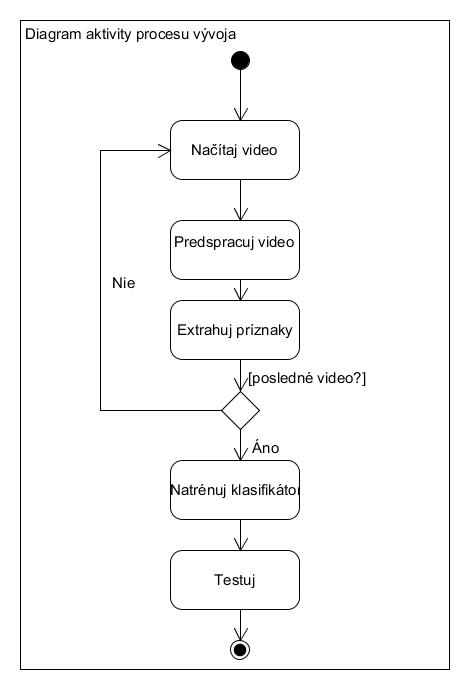
\includegraphics[width=10cm]{img/actTrenovanieKlasifikatora.jpg}
  \caption{Diagram plánu vývoja riešenia}
  \label{UML1}
\end{figure}

\subsection{Spôsob spracovania sekvencie}
Zo zadania vyplýva, že pre získanie príznakov z videa budeme potrebovať videosekvenciu rozdeliť na menšie časti, respektíve ju spracovať do formátu obrázku (.jpg, .png. alebo iné). Jednotlivé snímky z videa sú potrebné na hlbšiu analýzu. Podľa výberu datasetu budeme môcť zvoliť či budeme používať celú videosekvenciu, alebo iba jej časť, v ktorej je zrejmý druh pohybu. 

V jednotlivých triedach videí bude potrebné hľadať spoločné a rozdielne znaky na to, aby sme následne vybrali vhodný postup na spracovanie a získanie vhodných príznakov. Knižnica OpenCV neobsahuje metódy ktoré zabezpečia čítanie a prenos obrazu, avšak jej metódy využívajú funkcionalitu ďalšej knižnice FFmpeg, ktorá distribuuje prostredníctvom rozhrania jednotlivé obrazové snímky. 

\subsubsection{Získanie časovo-priestorových vzťahov}
Bude potrebné získať tieto vzťahy na porovnávanie s ďalšími videami, teda určenie vhodného spôsobu na získanie týchto vzťahov. Jedným zo spôsobov je napríklad algoritmus MHI (Motion History Image), ktorý nám môže zabezpečiť tieto príznaky z videa uložiť a ďalej spracovávať. Podľa tohto algoritmu by sme vedeli určiť odkiaľ kam sa aktér z videa pohyboval, akým spôsobom a rýchlosťou, čo môžme považovať za prvé vhodné príznaky pre určenie typu pohybu.\cite{c3} Tento algoritmus si bližšie popíšeme ďalej v tejto práci.

\subsubsection{Extrakcia príznakov}
Extrakcia príznakov je dôležitou časťou pre natrénovanie klasifikátora. Preto je potrebné vybrať príznaky, ktoré nám s čo najvyššou presnosťou zadefinujú konkrétny pohyb, ktorý sa bude vykonávať vo videu. Mali by to byť príznaky, ktoré sú jednoznačné a jedinečné pre každý z druhov pohybu. Preto musíme uvažovať vhodnú metódu extrahovania príznakov, aby sme zaistili diverzitu medzi triedami jednotlivých typov pohybu. K tomu nám bude nápomocná aj kombinácia viacerých spôsobov extrakcie. 

Tieto príznaky budeme extrahovať z predspracovaného zdroja a ukladať na disk pre natrénovanie klasifikátora, prípadne viacnásobné trénovanie a testovanie bude vhodné jednotlivé výsledky ukladať pre neskoršie porovnanie.

\subsubsection{Návrh klasifikátora}
Po úspešnom získaní príznakov z každej videosekvencie bude potrebné natrénovať klasifikátor tak, aby nám každá skupina spracovaných videozáznamov spadala do jednej triedy. Takto natrénovaný klasifikátor budeme potrebovať uložiť pre potreby testovania a porovnávania výsledkov a diverzity jednotlivých skupín. Zároveň budeme potrebovať zvoliť vhodný pomer dát na testovanie a tréning na základe datábáz, ktoré budeme mať k dispozícii. Z tohto dôvodu budeme potrebovať čo najviac videí, aby bol návrh klasifikačnej metódy čo najpresnejší.


\subsection{Databázy videí}
Na internete je veľké množstvo video databáz s rôznymi pohybmi objektov, ľudí a zvierat.
Výber databázy realizujeme na základe vlastností jednotlivých videí. Videá môžu byť snímané staticky z jedného miesta bez pohybu kamery, staticky s otáčaním kamery, taktiež dynamicky s rôznym pohybom a otáčaním kamery. Výber databázy bude najdôležitejšou súčasťou tejto práce, keďže od nej sa bude odvíjať celý ďalší postup.
\subsubsection{Vlastnosti videa} Dôležitými vlastnosťami videí z databáz sú:
\begin{itemize}
\item \textbf{rozlíšenie}
\item \textbf{dĺžka}
\item \textbf{počet videí}
\item \textbf{spôsob snímania}
\item \textbf{formát videa}
\item \textbf{počet objektov}
\end{itemize}

\textbf{Rozlíšenie} videa je dôležitým faktorom pre spracovnie z hľadiska kvality príznakov a snímkov. Zároveň jeho odporúčaná veľkosť sa líši od konkrétneho spôsobu extrakcie príznakov. Dôležité je, aby obraz konkrétnej aktivity na videu bol jasný a voľným okom rozpoznateľný.

\textbf{Dĺžka} sekvencie sa líši od rozmanitosti jednotlivých pohybov osoby. Niektoré databázy obsahujú videosekvencie s opakovaním pohybov, teda dĺžka videí v týchto databázach je väčšia ako tam, kde je daná aktivita alebo pohyb zachovaný bez opakovania.

\textbf{Počet videí} môže ovplyvniť výsledok a efektivitu rozpoznávania aktivít. Niektoré databázy obsahujú malé množstvo videí pre jeden konkrétny pohyb (okolo 10 až 20), iné zdroje videosekvencií ich majú aj viac ako 50 pre jeden typ pohybu.

\textbf{Spôsob snímania} v rozpoznávaní pohybu je dôležitou vlastnosťou, keďže nie všetky spôsoby riešenia je možné aplikovať na videá s pohybujúcou sa kamerou a opačne. 

\textbf{Formát videa} súvisí s jeho veľkosťou, avšak formát je možné meniť a konvertovať na nami potrebný rozmer.

\textbf{Počet objektov}, ktoré sa na videu pohybujú a vyhodnocujú vplýva na rozhodovanie, akými metódami sa bude riešiť detekcia a rozpoznávanie.

\subsubsection{Databázy ľudského pohybu}\label{dbludskeho}
Pre potrebu rozpoznávania pohybu osoby existuje viacero databáz, ktoré sme v našej práci uvažovali a testovali:
\begin{itemize}
\item \textbf{HMDB51}
\item \textbf{KTH}
\item \textbf{UCF-Sports}
\item \textbf{Hollywood}
\item \textbf{MSR Action I, II}
\item \textbf{IXMAS}
\item \textbf{WEIZMANN}
\end{itemize}

\textbf{HMDB51} je databáza pohybov v ktorej sa nachádza 51 tried pohybu a gestikulácie ako napríklad česanie vlasov, žuvanie, lezenie, potápanie, chôdza atď. Celkovo obsahuje 6849 videí s rozlíšením 320 x 240 pixelov. Videá sú so statickou aj dynamickou kamerou. Zdrojom videí je YouTube ako aj iné verejne dostupné databázy videí. Videá sú špecifické vysokou diverzitou kvality ako aj pohybu.\cite{c1}

\textbf{KTH} pohybová databáza so šiestimi triedami - chôdza, pomalý beh, beh, boxovanie, kývanie rukou, tlieskanie. V každej z týchto tried sa nachádza 100 čiernobielych videí s rozlíšením 160 x 120 pixelov so statickou kamerou. Videá sú natočené v interiéri ako aj exterieri. \cite{c1}

\textbf{UCF-Sports} obsahuje 9 tried pohybu so 182 videami so statickou aj dynamickou kamerou. Rozlíšenie videí je 720 x 480 pixelov. Videá sú z rôznych športových podujatí vysielaných v televízii - skok do vody, vzpieranie, jazda na koni a iné.\cite{c1} 

\textbf{Hollywood} databáza obsahuje 8 tried - vystúpenie z vozidla, bozkávanie, postavenie sa, sadnutie si a iné. Nachádza sa tam 430 videí s rozlíšením 300 - 400 x 200 - 300 pixelov s dynamickou kamerou a dynamickým pozadím.\cite{c1}

\textbf{MSR Action I, II} obsahujú 3 triedy pohybu so statickou kamerou a 16-timi videami s  rozlíšením 320 x 240 pixelov. Namodelované videá sú určené na detekciu pohybu, nie jeho rozpoznávanie. Vo videách sa nachádza viac ako jeden pohyb. V pozadí sa objavujú aj iné osoby, prípadne objekty ako auto. \cite{c1}

\textbf{IXMAS} alebo \textit{INRIA Xmas Motion Acquisition Sequences} obsahuje 13 tried s rozlíšením 390 x 291. Pohyb je zaznamenávaný z viacerých statických kamier. \cite{c1}

\textbf{WEIZMANN} obsahuje 10 tried pohybu, celkový počet videí je 90. Obsahujú triedy pohybu ako chôdza, beh, kývanie jednou alebo dvomi rukami, skok na mieste a iné. Videá sú natočené so statickou kamerou a pozadím  v interiéri  s rozlíšením 180 x 144. \cite{c1}

\subsection{Postup spracovania obrazu}
Na získanie príznakov a potrebu klasifikácie pohybu analyzujeme a zvažujeme konkrétne spôsoby spracovania obrazu z videa. Pre tento účel berieme v úvahu algoritmus \acrfull{mhi} na extrakciu prvotných príznakov a následné spracovanie pomocou \acrfull{hog}. 

Pre zaistenie najvhodnejších príznakov a zaručenie vyššej úspešnosti klasifikácie uvažujeme použitie \acrfull{pca}, ktoré môže urýchliť trénovanie klasifikátora, ak sa počet dimenzií zredukuje. Takto získané príznaky by sme následne vedeli natrénovať pomocou \acrfull{svm}. Z natrénovanej SVM vieme otestovať úspešnosť klasifikátora, ktorý sme získali a tým sa dostať ku výsledkom a porovnávaniam. 

\subsubsection{Motion History Image} \label{MHIlabel}
\acrshort{mhi} je metódou, ktorá je založená na časovej šablóne. Je to jednoduchá metóda avšak robustná, vhodná na reprezentovanie a analýzu pohybu.\cite{c3}  Táto metóda bola prvýkrát popísaná v dokumente \textit{``An appearance-based representation of action''} od Aarona Bobicka a Jamesa W. Davisa.\cite{c2} Rozpoznávanie akcie pomocou MHI patrí do skupiny prispôsobovania šablóny. V MHI sa informácia pohybu v čase spája do jednej dátovej matice, kde intenzita pixelov je funkciou histórie pohybu na danej pozícii pixelu. MHI sa vypočítava pomocou aktualizačnej funkcie.\ref{MHIeq}

\begin{figure}[H]
  \centering
  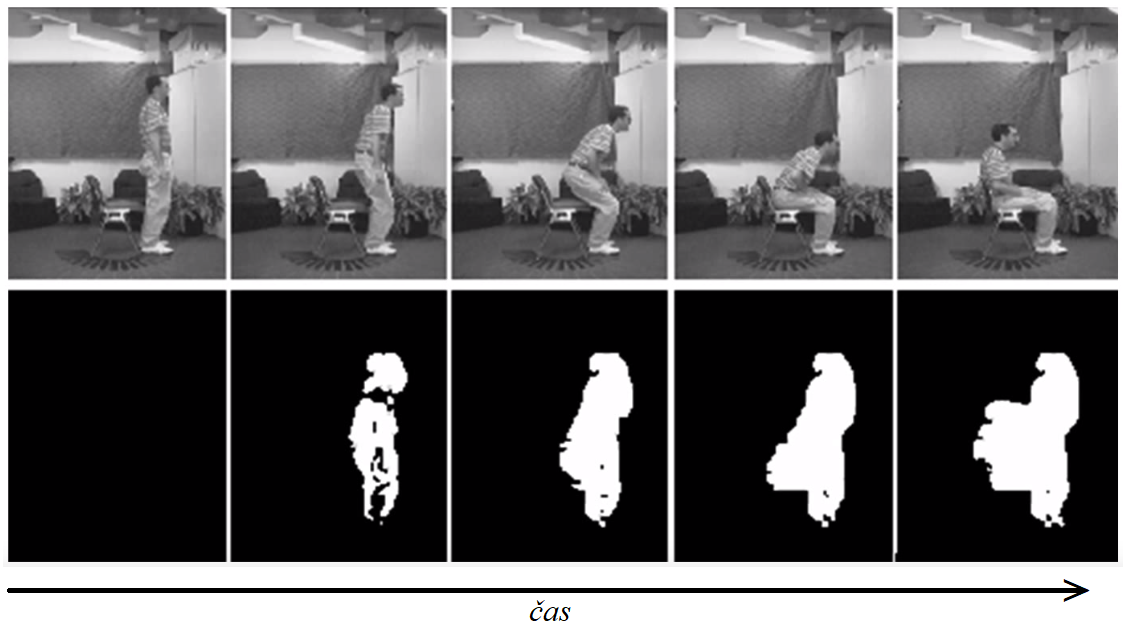
\includegraphics[width=16cm]{img/MHIudacity.png}
  \caption{Priebeh videa a tvorba MEI \cite{c22}}
  \label{MHIuda}
\end{figure}

Na obrázku \ref{MHIuda} v spodnej časti môžme vidieť MEI \textit{(Motion Energy Image)}, čo je základom pre vytváranie MHI. Jednotlivé snímky sú zoradené v čase akom boli nasnímané. V hornom riadku obrázkov vidíme neupravené snímky. Obrázky MEI sa kumulatívne spájajú do jedného obrazu. Nenesú informáciu o histórii daného pohybu, iba o tom, ktoré pixely sa menili a kde sa pohyb konal. Pridaním tmavnutia pixelov je možné vytvoriť MHI z \acrshort{mei}.

Z tohto riešenia je možné jednoducho odvodiť riešenie MHI, kde pri kumulovaní jednotlivých snímkov do jedného je uberaná intenzita všetkých pixelov v každej iterácii. Tento proces je zapísaný rovnicou na obrázku \ref{MHIeq}.

\begin{figure}[H]
  \centering
  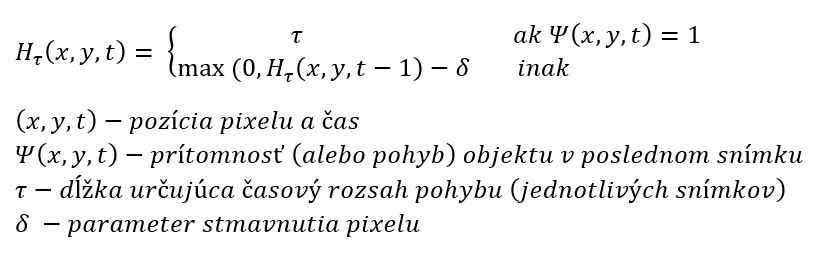
\includegraphics[width=14cm]{img/MHIeq.jpg}
  \caption{Funkcia zmeny pixelov v MHI}
  \label{MHIeq}
\end{figure}

Táto aktualizačná funkcia je volaná pre každý ďalší snímok, ktorý analyzujeme z videosekvencie. Výsledkom tohto výpočtu je skalárny snímok, v ktorom svetlejšie časti obrázku označujú najnovšie menené pixely a tmavšie sú tie, ktoré boli menené dávnejšie z pohľadu pohybu na videu.

To nám umožňuje zaznamenať pohyb z videa do jediného obrázku, v ktorom je vystihnutý celý priebeh videa alebo jeho časti. Táto technika je vhodná na použitie pri videách so statickou kamerou a pozadím.\cite{c10}

\begin{figure}[H]
  \centering
  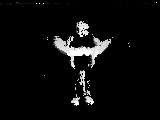
\includegraphics[width=13cm]{img/MHIclap.jpg}
  \caption{Motion History image tlieskania}
  \label{MHIclap}
\end{figure}

Na obrázku \ref{MHIclap} je príklad spracovaného pohybu z videa do MHI, na ktorom môžme vidieť pohyb tela pri akcii tlieskania.

\subsubsection{Histogram of Oriented Gradients} \label{HOGlabel}
Deskriptor vlastností je forma reprezentácie obrazu alebo jeho časti, ktorá zjednodušuje obraz extrakciou dôležitých informácií. Tento deskriptor premieňa obraz na pole, resp. vektor vlastností, v ktorom sa nachádzajú

Tento deskriptor je užitočný  pre potreby detekcie a rozpoznávania obrazu, kde jeho vektor môže byť vstupom pre klasifikačné algoritmy ako napríklad SVM. 

HOG deskriptor (Histogram of oriented gradients) používa ako vektor príznakov rozdelenie smerov orientovaných gradientov. Tieto príznaky sú veľmi dobré na detekovanie hrán v obraze a poskytujú vhodné informácie o jeho vlastnostiach.

\paragraph{Predpríprava a výpočet gradientu}

Vo väčšine prípadov je potrebné orezať obraz na časť, ktorú potrebujeme analyzovať s tým, že pomer jeho strán musí byť počas zmenšovania a orezávania zachovaný. 

Na výpočet HOG deskriptora je najprv nutné vypočítať horizontálne a vertikálne gradienty, následne je možné vypočítať histogram gradientov. Tento krok je jednoduché dosiahnuť pomocou filtrovania obrazu nasledovnými jadrami.

\begin{figure}[H]
  \centering
  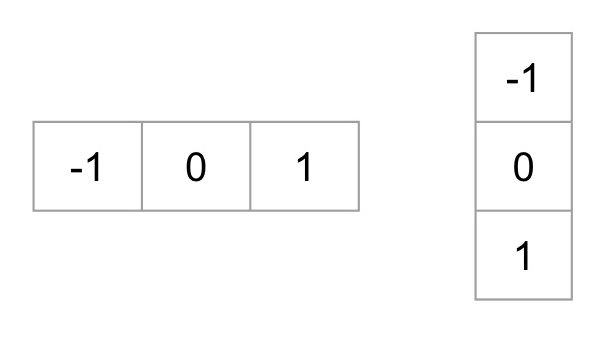
\includegraphics[width=12cm]{img/HOGkern.png}
  \caption{Jadrá pre výpočet gradientov \cite{c20}}
  \label{HOGkern}
\end{figure}

Ďalej potrebujeme nájsť veľkosť a smer gradientov pomocou nasledovných vzťahov:

\begin{figure}[H]
  \centering
  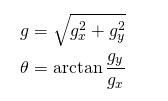
\includegraphics[width=5cm]{img/HOGfunc.png}
  \caption{Výpočet veľkosti a smeru gradientu \cite{c20}}
  \label{HOGfunc}
\end{figure}

Kde $g$ je veľkosť gradientu a  $\theta$ je jeho smer.  $x,y$ sú osi jednotlivých gradientov, od ktorých sa odvíjajú. 

Na obrázku bežca si ukážeme, ako takéto gradienty po výpočte vyzerajú.

\begin{figure}[H]
  \centering
  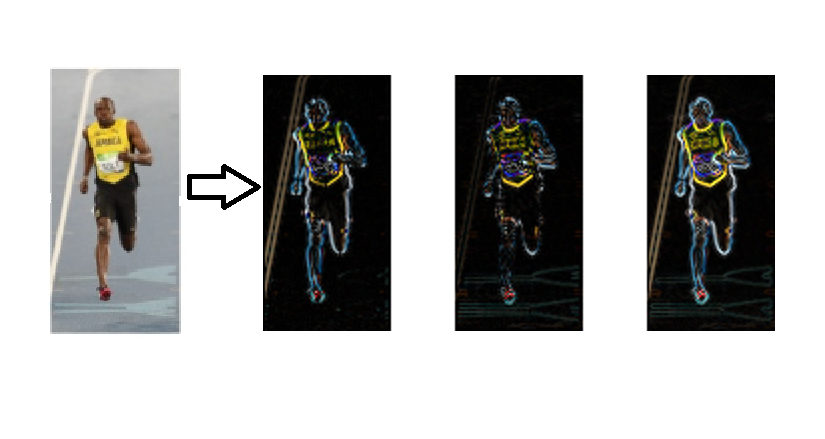
\includegraphics[width=16cm]{img/HOGboltg.png}
  \caption{Originálny obraz transformovaný na gradienty \cite{c20}}
  \label{HOGbolt}
\end{figure}

Na obrázku \ref{HOGbolt} môžme vidieť transformáciu originálneho obrazu na absolútnu hodnotu gradientu osi x, vedľa nej absolútnu hodnotu gradientu y a napravo veľkosť gradientu.
Gradient osi x na obrázku zaznamenal vertikálne čiary bežeckej trate, gradient osi y zase horizontálne hodnoty. Veľkosť gradientu zaznamenáva každú ostrú zmenu intenzity jednotlivých pixelov. Pokiaľ sú časti obrazu plynulé, žiadne dôležité informácie nie sú zachytené. 
Obraz gradientu eliminuje nedôležité informácie v obraze, čo môžme demonštrovať tým, že aj na takomto obraze gradientov môžme rozpoznať, že ide o bežiacu osobu.

\paragraph{Výpočet gradientov po bunkách}

V tomto kroku môžme obraz rozdeliť do buniek o veľkosti  8 x 8 pixelov, pre ktoré bude histogram gradientov počítaný osobitne pre každú bunku.

Výpočet po bunkách je dôležitým krokom na redukovanie objemu dát, pretože pre každý pixel v bunke máme dokopy\textit{ 8x8x3 }(192) a zároveň \textit{8x8x2 (veľkosť a smer gradientu)} (128). Ukážeme si, že pomocou redukcie uhlov do 9tich smerových kategórií vieme týchto 128 hodnôt uložiť ako 9 hodnôt. Reprezentácia takýmto spôsobom je kompaktnejšia, zároveň je odolnejšia voči šumu v obraze. 

Histogram gradientu je vlastne vektor deviatich smerových kategórií, ktoré zoskupuje podľa uhla, ktorý gradient má. 

\begin{figure}[H]
  \centering
  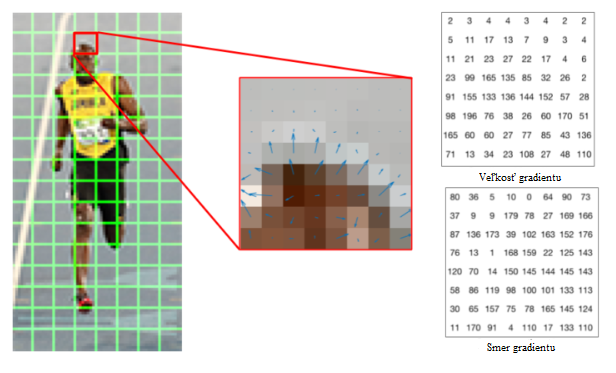
\includegraphics[width=16cm]{img/HOGgrad.png}
  \caption{Príklad veľkostí a smerov gradientov \cite{c20}}
  \label{HOGgrad}
\end{figure}
Na obrázku \ref{HOGgrad} môžme vidieť znázornenie vypočítaných hodnôt gradientu bunky \textit{8 x 8}. Na obrázku v strede môžme vidieť jednotlivé pixely obrázku a gradienty, ktoré majú svoju veľkosť a smer. Na pravej strane obrázku hore sú veľkosti gradientov jednotlivých pixelov a dole sú ich smery v stupňoch. Stupne sú určené v rozmedzí 0 - 180 (bezznamienkový), aj keď je možné využiť aj interval 0 - 360 stupňov (znamienkový) . To všetko závisí od toho, či používame gradienty so znamienkom alebo bez. Výhodou používania 180 stupňového intervalu je, že bezznamienkové gradienty sú úspešnejšie pre potreby detekcie pohybu osoby. 

Ďalším krokom je vytvorenie HOG v konkrétnych bunkách napríklad o rozmere \textit{8 x 8}. Histogram bude obsahovať 9 skupín pre každý 20-ty stupeň z rozmedzia 0 - 180 stupňov \textit{( 0, 20, 40, 60 ... 160)}. 

Následne sa rozdeľovanie do jednotlivých skupín prebieha ako na obrázku \ref{HOGbins}. 

\begin{figure}[H]
  \centering
  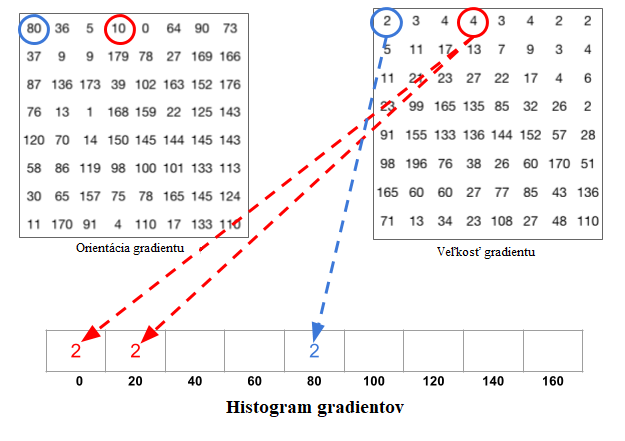
\includegraphics[width=16cm]{img/HOGbins.png}
  \caption{Rozdeľovanie veľkostí gradientov podľa orientácie \cite{c20}}
  \label{HOGbins}
\end{figure}


Môžme vidieť, že skupina kam ide veľkosť gradientu sa vyberá podľa  jeho orientácie. Gradient v modrom je zaradený do skupiny 80 pretože má orientáciu 80 stupňov a je priradená hodnota 2, pretože je to jeho dĺžka. Pri gradiente v červenom kruhu je hodnota rozdelená medzi skupiny 0 a 20, keďže orientácia gradientu je 10, rozdelí sa veľkosť na dve rovnaké časti. V prípade, že by sme mali orientáciu gradientu 170 stupňov s veľkosťou 85, rozdelila by sa jeho veľkosť medzi skupinu 0 a 160 taktiež v pomere 1:1.
Takto máme vytvorený prvý histogram.



\paragraph{Normalizácia blokov}
Normalizovanie blokov je potrebné na to, aby bol deskriptor nezávislý na zmene svetelnosti obrazu. Takáto normalizácia sa vypočíta následovne

\begin{figure}[H]
  \centering
  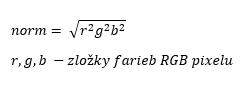
\includegraphics[width=6cm]{img/HOGL2.png}
  \caption{Výpočet L2 normy\cite{c20}}
  \label{HOGL2}
\end{figure}

Takto vypočítaná hodnota sa nazýva \textit{L2-norma}. Vydelené zložky RGB pixelu touto normou sú normalizované, teda z intervalu \textit{<0,1>}. Teda to nám eliminuje zmeny hodnôt pre pixely, ktoré boli napríklad dvojnásobne zosvetlené. 

Tak ako sme normalizovali každú zložku, je potrebné normalizovať aj zložky celého histogramu. Na to sa používa normalizácia väčších blokov aj s prekrytím \footnote{napríklad veľkosť bloku je 16 a posun bude po 8 pixelov}. 

Z takto získaných príznakov vieme získať finálny HOG vektor príznakov tým, že spojíme čiastkové vektory.
\cite{c11}\cite{c20}


\subsubsection{Principal Component Analysis} \label{PCAlabel}
Analýza hlavných komponentov (angl. Principal Components Analysis) je metóda štatistiky, ktorá využíva ortogonálnu transformáciu za účelom zmeny prvkov, v ktorých sa vyskytuje korelácia na prvky, kde  sa takáto lineárna korelácia nebude nachádzať. \acrshort{pca} teda spracováva a upravuje jednotlivé komponenty tak, aby sa ich dimenzia zmenšila, alebo bola nanajvýš rovnaká a zároveň sa snaží zachovať čo najväčšie množstvo informácií o pôvodných premenných. Tento prístup pomáha analyzovať dané dáta v podpriestore, čo nám umožňuje ďalšie spracovanie.

Dôležitou súčasťou v PCA sú vlastné vektory. Sú to nenulové vektory, ktorých smer sa po transformácii pomocou lineárneho operátora nemení, pojem vlastný vektor v PCA obmieňame za hlavný komponent. 

V počítačovom videní má táto metóda veľmi dobrý vplyv na dáta charakterizujúce rôzne špecifické tvary, objekty, keďže nám umožňuje zosilniť význam príznakov, ktoré sú pre daný problém dôležité, a tie, ktoré nie sú potrebné, dokáže eliminovať. Táto transformácia teda zvyšuje varianciu hlavných komponentov naprieč všetkými lineárnymi kombináciami vektora, čo napomáha zvyšovať úspešnosť klasifikátora pri riešení rozpoznávania na extrakciu príznakov. Túto metódu navrhol v roku 1901 matematik anglického pôvodu Karl Pearson. Jej rôzne obmenené a vylepšené verzie sa využívajú dodnes v štatistike, \textit{počítačovom videní}, robotike a ďalších smeroch.


\paragraph{Variancia}
Variancia kóduje informácie, ktoré obsahujú jednotlivé dáta. V dvojrozmernom priestore je potrebné pre \textit{n} bodov mať \textit{2n} čísel, ktoré nám reprezentujú tieto dáta. Na obrázku \ref{PCAgraph} môžme vidieť dva smery maximálnej variancie. Modrá čiara reprezentuje smer, kde je najviac informácií, tento smer je prvý hlavný komponent. Druhý hlavný komponent, ktorý je označený zelenou farbou, je smer variancie kolmý na smer prvého hlavného komponentu, kde je v tomto smere najväčší rozptyl dát. V 2D priestore existujú iba dva hlavné komponenty. Koľko dimnezií má priestor, toľko môže byť maximálne množstvo hlavných komponentov.  

\begin{figure}[H]
  \centering
  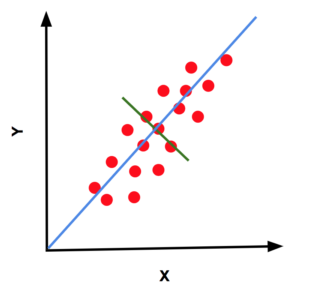
\includegraphics[width=6cm]{img/PCAgraph.png}
  \caption{HLavné komponenty v grafe \cite{c21}}
  \label{PCAgraph}
\end{figure}

\paragraph{Redukcia dimenzie}
Hlavným cieľom PCA je redukcia dimenzie. TO znamená, že dáta z 3D priestoru chceme reprezentovať v dvojrozmernom priestore. Princíp spočíva v tom, že ak máme  3D priestor s tromi hlavnými komponentami, môžme zarovnať osi tohto priestoru podľa hlavných komponentov, čím reprezentujeme tie isté dáta v inom súradnicovom systéme. Ak odstránime dimenziu, kde je tretí a teda najmenší hlavný komponent, stále nám ostanú dva hlavné komponenty s relevantnými dátami na ich reprezentáciu. Tento prístup napomáha pri vysokom počte dimenzií. Znížením dimenzie je možné filtrovať dátový šum a tak získať presnejší výsledok. 

\paragraph{Vlastné vektory a hodnoty matice}
Vlastný vektor matice je vektor, ktorého smer sa pri násobení nemení. 
Teda platí $ Av = \lambda v $ kde $A$ je matica,  $v$ je vektor a  $\lambda$ je skalárna veličina (číslo).

Pri takomto násobení sa mení veľkosť vektora $v$ a smer ostáva zachovaný.

\paragraph{Výpočet PCA}
Pre výpočet PCA je potrebné vložiť vytvorené dátové body do matice, v ktorej každý stĺpec reprezentuje jeden dátový bod. Teda pre trojrozmerný priestor, kde je \textit{n} bodov bude mať matica \textit{3} stĺpce a \textit{n} riadkov ako na obrázku \ref{PCAdatamx}. 

\begin{figure}[H]
  \centering
  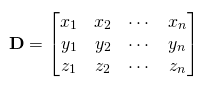
\includegraphics[width=6cm]{img/PCAdatamx.png}
  \caption{3D matica dát \cite{c21}}
  \label{PCAdatamx}
\end{figure}

Po vytvorení takejto matice je potrebné vypočítať priemer všetkých dátových bodov, teda koľko rozmerov, toľko priemerov. Tie sa vypočítajú ako súčet všetkých hodnôt v rozmere vydelený ich počtom. \ref{PCAmean}

\begin{figure}[H]
  \centering
  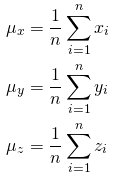
\includegraphics[width=3cm]{img/PCAdatamean.png}
  \caption{Výpočet priemerov dátových bodov\cite{c21}}
  \label{PCAmean}
\end{figure}

Na základe priemeru sa vytvorí matica, v ktorej hodnoty sa vypočítajú ako hodnota v matici \textit{D} zmenšená o hodnotu priemeru \ref{PCAdatamx2}. Po získaní tejto matice môžme získať jednoducho kovariančnú maticu, z ktorej vieme získať roztyl dát. Diagonála kovariančnej matice obsahuje variancie osí X, Y a Z, hodnoty mimo diagonály určujú kovarianciu medzi dvomi dimenziami (X, Y alebo Y, Z alebo Z, X). 

\begin{figure}[H]
  \centering
  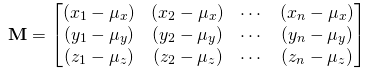
\includegraphics[width=9cm]{img/PCAdatamx2.png}
  \caption{3D matica priemerov\cite{c21}}
  \label{PCAdatamx2}
\end{figure}

Kovariančná matica sa vypočíta ako $C = MM^T$, kde $M^T$ je transponovan8 matica $M$. Rozmer matice \textit{C} je \textit{m * m}, kde \textit{m} je počet dimenzií.


\begin{figure}[H]
  \centering
  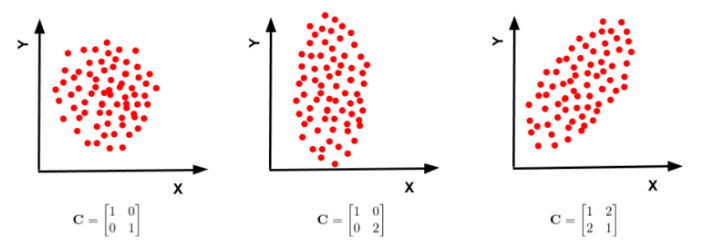
\includegraphics[width=17cm]{img/PCAdatacompare.png}
  \caption{Porovnanie kovariančných matíc pre rôzne rozptyly dát\cite{c21}}
  \label{PCAcmp}
\end{figure}

Na obrázku \ref{PCAcmp} môžme vidieť ako sa mení kovariančná matica v závislosti od rozptylu dát.
Na prvej časti obrázku sú dáta rozptýlené rovnako všetkými smermi, teda kovariančná matica má na diagonále rovnaké hodnoty. Na strednom obrázku môžme vidieť, že hodnoty sú natiahnuté v smere osi \textit{y}, diagonála kovariančnej matice nemá rovnaké hodnoty. Na poslednej časti obrázku sú hodnoty rozptýlené v 45-stupňovom uhle, diagonálne hodnoty kovariančnej matice sú rovnaké ako aj hodnoty mimo diagonály.\cite{c21}


\subsubsection{Support Vector Machine} \label{SVMlabel}
SVM je metóda strojového učenia s učiteľom, je vhodná na používanie pri klasifikácii alebo regresnej analýze. Táto metóda na základe trénovacích vzoriek, ktoré sú priradené do jednej z dvoch tried vytvorí model. Tento model je následne schopný priraďovať nové vzorky do jednej z týchto tried, čo z neho robí nepravdepodobnostný binárne lineárny klasifikátor. SVM model reprezentuje vzorky ako body v priestore, tak, že mapuje jednotlivé vstupy do kategórií, ktoré sú v tomto priestore jasne oddelené. Klasifikátor priraďuje nové vzorky podľa toho, ku ktorej z tried majú bližšie v rámci tohto priestoru.

Okrem lineárnej klasifikácie je SVM schopné efektívne riešiť aj nelineárne separovateľné problémy pomocou takzvaného jadrového triku \textit{(angl. Kernel trick)} tým, že rozšíri dimenzionalitu dát. Pokiaľ dáta nie sú pri trénovaní označené, do ktorej kategórie patria, učenie s učiteľom nie je možné, avšak je možné učenie bez učiteľa tak, že algoritmus sa snaží nájsť prirodzené zoskupenie dát a tak ich rozdeliť do kategórií.

Medzi najčastejšie používané jadrové funkcie patria:

\begin{itemize}
\item \textbf{Polynóm stupňa \textit{p}}
\item $  K(x,y) = (x.y + 1)^p $
\item \textbf{Radiálne bázové funkcie}
\item $   K(x,y) = e^{(-\|x-y\|^2/2\sigma^2)}  $
\item \textbf{Dvojvrstvová neurónová sieť }
\item $   K(x,y) = \tanh(\kappa x.y - \delta)  $
\end{itemize}

SVM algoritmus vytvorili Hava Siegelmann a Vladimir Vapnik. Tento algoritmus má široké využitie a je používaný v priemyselných aplikáciách, počítačovom videní, umelej inteligencii.  \cite{c7}

\paragraph{Definícia algoritmu}
SVM vytvára hyperrovinu \footnote{Podpriestor, ktorý má o jednu dimenziu menej ako priestor, v ktorom sa nachádza.}, alebo viacero hyperrovín, vo vysokorozmernom priestore, ktorý môže byť použitý na klasifikáciu, regresiu alebo iné úlohy. Dobrá separácia sa dosiahne vtedy, keď hyperrovina má veľkú vzdialenosť od najbližšieho trénovacieho bodu akejkoľvek triedy. Teda platí, čím je väčšia vzdialenosť hyperroviny od trénovacích údajov, tým je nižšia chyba klasifikátora pri určovaní triedy testovacej vzorky.\cite{c12}

Keďže nie všetky problémy je možné lineárne separovať, bolo navrhnuté, aby sa priestor, ktorý SVM spracováva rozvrhol do viacrozmerného priestoru, čo uľahčí rozdelenie jednotlivých dát do tried. Pre zanechanie výpočtovej rýchlosti je mapovanie v SVM navrhnuté v pôvodnom priestore, kde sa následne zvolí vhodná jadrová funkcia $ k(x,y)$ . 
Hyperroviny vo viacrozmernom priestore sú definované ako súbory bodov, kde ich vektory majú konštantnú dĺžku. Následne body z priestoru príznakov sú mapované do hyperroviny. 

\paragraph{Lineárny klasifikátor}
Najjednoduchšou možnosťou použitia SVM je prípad lineárneho klasifikátora pre dáta, ktoré je možné lineárne rozdeliť do dvoch tried pomocou hyperroviny. Príklad takéhoto problému je na obrázku \ref{LinSep}.

\begin{figure}[H]
  \centering
  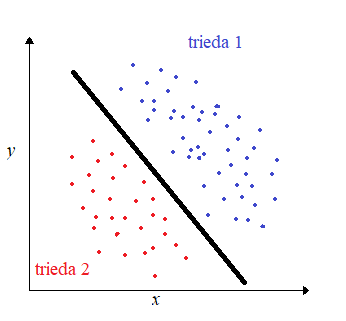
\includegraphics[width=10cm]{img/linsep.png}
  \caption{Príklad lineárne separovateľného problému}
  \label{LinSep}
\end{figure}


\paragraph{Nelineárny klasifikátor}
Na obrázku č. \ref{SVMobr} môžme vidieť lineárne neseparovateľný problém dvoch množín, ktorý sa po pridaní tretej dimenzie stáva lineárne separovateľný. Takýmto spôsobom dokážeme s SVM zatriediť jednotlivé videá z množín do správnych tried. Pomocou jadrového triku vieme lineárne separovať aj lineárne neseparovateľné problémy.\cite{c12}

\begin{figure}[H]
  \centering
  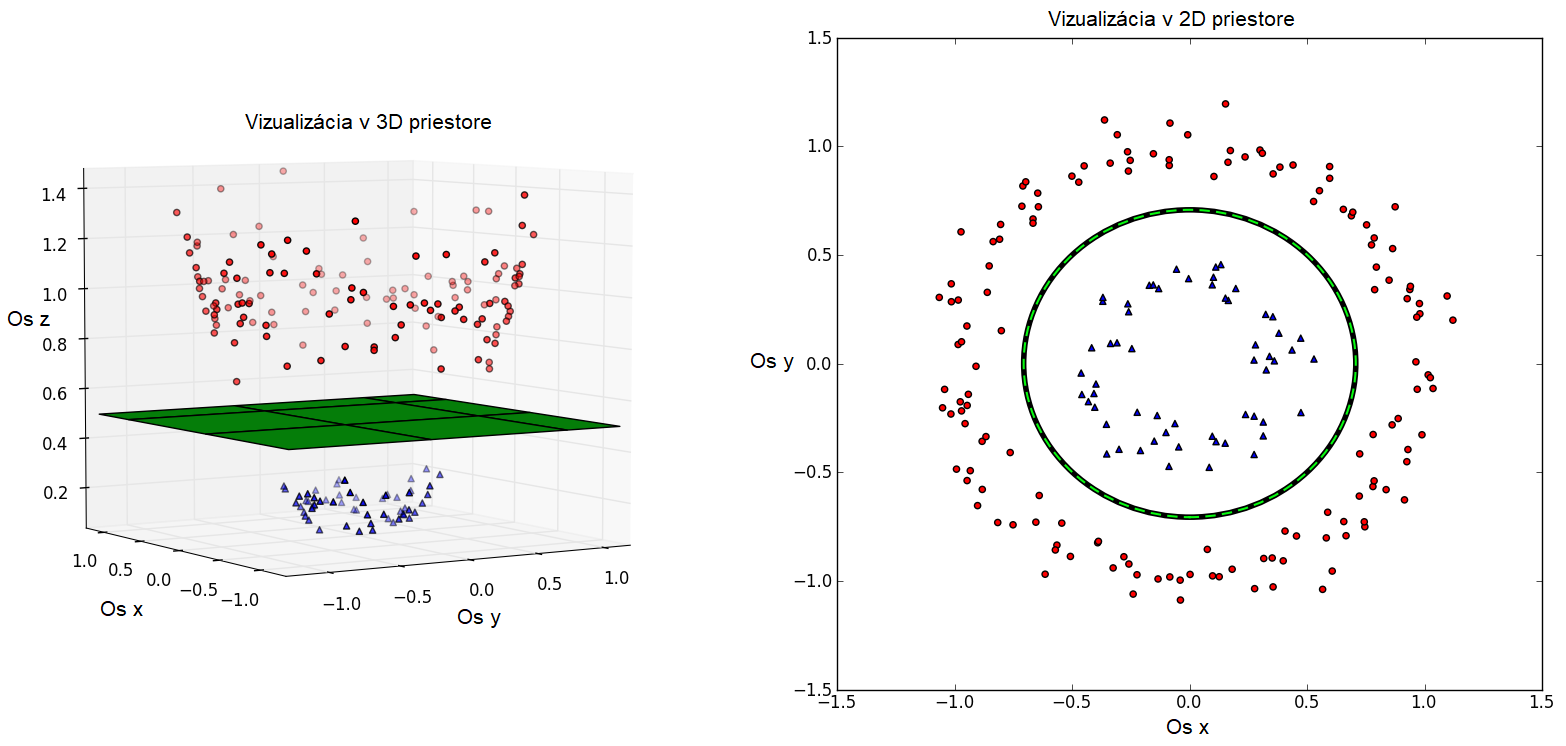
\includegraphics[width=16cm]{img/SVM.png}
  \caption{Rozšírenie dimenzie v SVM}
  \label{SVMobr}
\end{figure}

\newpage

\section{Návrh riešenia}
Po oboznámení s teoretickými piliermi tejto práce prejdeme ku konkrétnemu riešeniu témy a implementácii, ktorú sa nám podarilo vytvoriť. Postupne prejdeme jednotlivé kroky vytvárania programu od analýzy datasetov, načítavania a ukladania videosekvencií do obrazových formátov. Ďalej si ukážeme metódy a spôsoby, ktorými sme následne vzniknuté dáta spracovali pre potrebu výberu príznakov a zatriedenia do jednotlivých tried. Fungovanie programu priblížime aj časťami kódu s popisom, na čo slúži a ako pracuje. Súčasťou tejto kapitoly bude aj krátky popis zmien, ktoré sme počas návrhu tejto implementácie vykonali a samozrejme aj ich dopad na finálne riešenie.

\subsection{KTH Databáza}
Pre naše riešenie sme vyberali z viacerých datasetov, ktoré boli popísané v kapitole \ref{dbludskeho}. Nakoniec sme sa rozhodli pre databázu KTH, v ktorej máme 6 tried pohybu a nachádza sa pri každom z nich 100 videí. Naše rozhodnutie sme učinili takto z viacerých dôvodov. Potrebovali sme dataset, v ktorom sa nachádza veľké množstvo videí, zároveň vo videách sme potrebovali statickú kameru so statickým pozadím, aby sme predišli zvýšenému šumu. V tejto databáze sú pohyby:

\begin{itemize}
\item Boxovanie
\item Mávanie rukami
\item Tlieskanie rukami
\item Beh
\item Pomalý beh
\item Chôdza
\end{itemize}

Pri analýze snímkov sme zistili, že dĺžka videí je od \textit{\textbf{8 do 59 sekúnd}}. Čo pre dané typy pohybov je postačujúci čas na to, aby sme z nich dokázali extrahovať dôležité informácie, ktoré sa tohto pohybu týkajú.  Počet snímkov za sekundu v každom z videí je 25, z tohto dôvodu sme usúdili, že aj v prípade krátkeho videa s dĺžkou 8 sekúnd budeme mať k dispozícii minimálne \textit{\textbf{200}} snímkov. Ďalším dôležitým faktom je, že sa budeme musieť popasovať s podobnosťou pohybov behu, pomalého behu a chôdze, keďže sú veľmi podobné, a ich rozdiel je iba v rýchlosti vykonávania. Je nutné dodať, že v každom z videí sa jednotlivé typy pohybov opakovali viacnásobne, z čoho sme už vopred usudzovali, že na spracovanie nám bude stačiť iba časť videa, čo nám ušetrí čas spracovania dát počas behu programu. 

\begin{figure}[H]
  \centering
  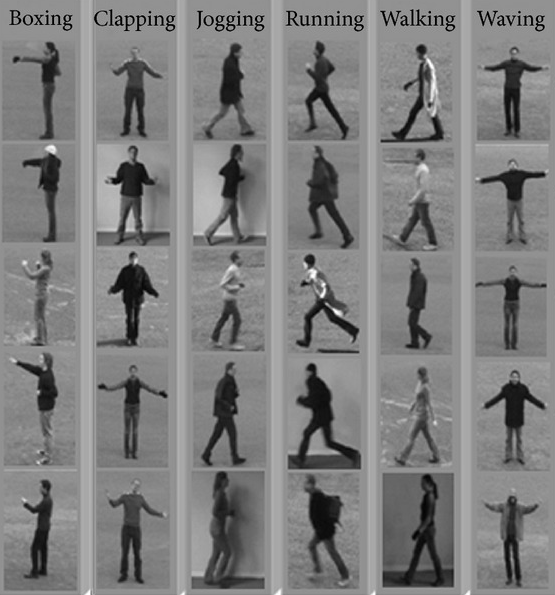
\includegraphics[width=10cm]{img/KTHdataset.png}
  \caption{Jednotlivé pohyby v datasete KTH \cite{c14}}
  \label{KTHobr}
\end{figure}

Na obrázku \ref{KTHobr} vidíme všetky kategórie pohybov, jednotlivé pohyby vykonáva viacero osôb rôznymi spôsobmi, teda je medzi týmito pohybmi aj diverzita, ktorá je určite vhodná na trénovanie pohybu. 

\subsection{Predspracovanie videa}
Na predspracovanie videa a vytiahnutie prvotných príznakov sme sa rozhodli z našich videí vytvoriť obrázky, na ktorých sa bude nachádzať história pohybu. Algoritmus MHI, ktorý sme pri tom použili sme popísali v časti \ref{MHIlabel}. Tento algoritmus sme zvolili na základe toho, že máme databázu videí bez pohyblivého pozadia, teda predídeme šumom na pozadí a budeme sa môcť venovať iba pixelom, ktoré menia svoju pozíciu v rámci videa. Presne to je postačujúca podmienka na to, aby sme bez väčších problémov mohli implementovať funkcionalitu algoritmu MHI na nami zvolený dátový rozsah. Vytvoriť MHI sme sa rozhodli zo všetkých videí, aby sme následne videli, akým spôsobom prebehlo spracovanie, či je možné z MHI vyčítať pohyb a jeho základné znaky. 

\begin{figure}[H]
  \centering
  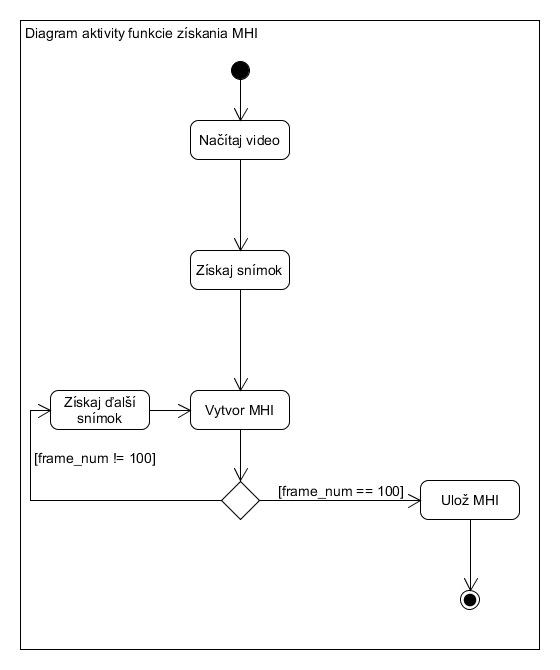
\includegraphics[width=17cm]{img/actMHIsnimok.png}
  \caption{Diagram aktivity získania MHI}
  \label{MHIcreate}
\end{figure}  


V tejto ukážke \ref{MHIcreate} diagramu aktivít je znázornený proces získavania MHI snímky z našej implementácie. Prvým krokom je načítanie videa, z ktorého následne vyberáme po jednom obrázku. Z každého obrázku vytvárame MHI z predchádzajúcich snímkov. V tomto konkrétnom prípade opakujeme cyklus dovtedy, kým nezískame MHI zo snímku číslo 100, ktoré predstavuje štvrtú sekundu pohybu (25 snímkov za sekundu). V prípade, že nám príde snímok číslo 100, prejdeme na jeho uloženie na lokálny disk, kde bude pripravený na ďalšie spracovanie. 

\begin{figure}[H]
  \centering
  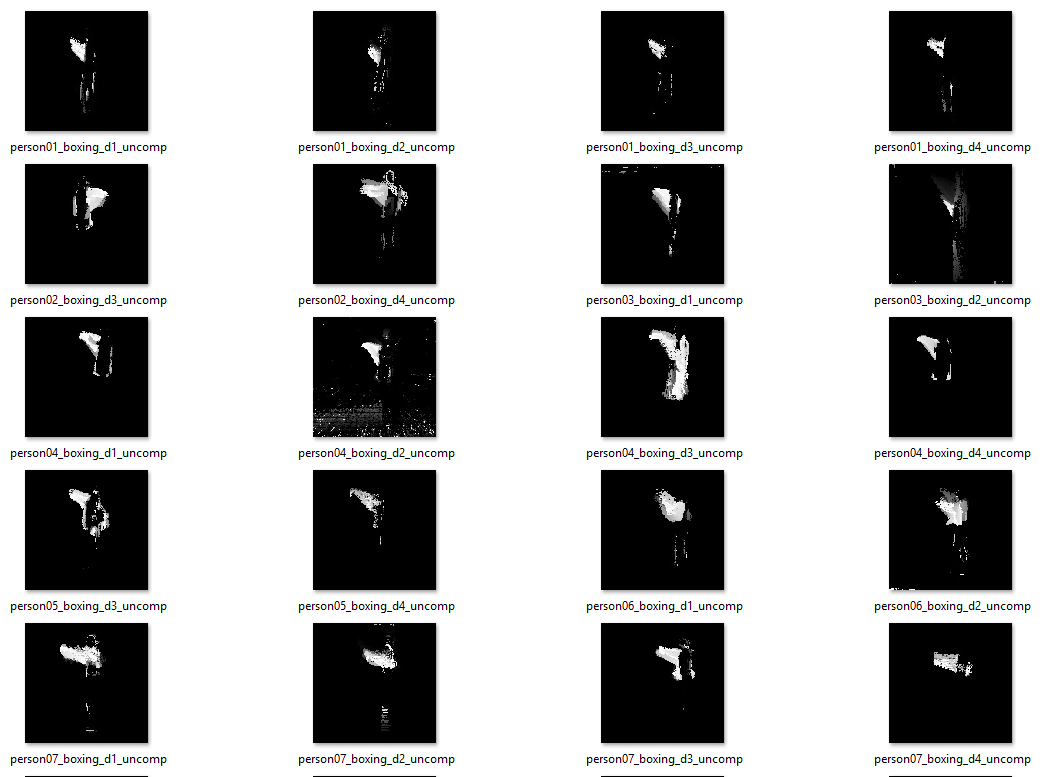
\includegraphics[width=16cm]{img/MHIbox.png}
  \caption{Predspracované videá boxu.}
  \label{MHIbox}
\end{figure}  

Na obrázku \ref{MHIbox} môžme vidieť príklad už predspracovaných MHI prostredníctvom nášho algoritmu. Takto sme si vytvorili všetkých 600 obrázkov z pohybov na ďalší výber príznakov, ktoré sme uložili podľa typu pohybu do jednotlivých priečinkov s ich názvami. 

\subsection{Výber príznakov}
Keďže už máme predspracovaný obraz vo forme MHI, môžme pokračovať v extrahovaní príznakov z týchto obrazov. Na tento účel sme zvolili deskriptor HOG popísaný v časti \ref{HOGlabel}. Týmto spôsobom vytvoríme vektor príznakov, ktorý budeme môcť následne spracovať prostredníctvom PCA a tak ho dať trénovať do klasifikátora pre každý jeden pohyb z trénovacej množiny. Príznaky z každého MHI obrázku by mali byť v tvare vektora konštantnej dĺžky. 

\subsubsection{Príznaky HOG} \label{HOGim}

V našom algoritme na získanie HOG príznakov vstupuje do funkcie \textit{hogCreate} parameter \textit{image} je vlastne obrázkom, ktorý je výstupom funkcie   \textit{imread} z knižnice OpenCV. Pre dobré vybratie príznakov je potrebné nastaviť a vytvoriť \textit{HOGDescriptor}, ktorý obsahuje viacero parametrov:

\begin{itemize}
\item winSize
\item blockSize
\item blockStride
\item cellSize
\item nbins
\item gammaCorrection
\item nlevels 
\end{itemize}

\textbf{winSize} parameter určuje veľkosť okna na detekciu, musí byť zarovnaný podľa \textit{blockStride} a \textit{blockSize}.

\textbf{blockSize} je veľkosť bloku v pixeloch. Má byť zarovnaný na veľkosť bunky \textit{cellSize}.

\textbf{blockStride} musí byť násobkom veľkosti bunky, znamená veľkosť kroku, ktorým sa blok bude posúvať.

\textbf{cellSize} je veľkosť bunky.

\textbf{nbins} je počet rozdelení uhlov do ktorých jendotlivé gradienty zapadajú.

\textbf{gammaCorrection} hodnota určuje, či sa má použiť predspracovanie gamma úpravy alebo nie.

\textbf{nlevels} určuje maximálny počet detekčných okien, predvolená hodnota je 64.

Po takomto nastavení deskriptora HOG môžme následne spracovať vstupný obraz a vytvoriť tak histogram hodnôt, ktoré už sú reprezentovateľné príznaky, ktoré vložíme do vektora príznakov \textit{arrVectorFinal}. Konečným výstupom je teda pole vektorov, ktoré obsahuje príznaky extrahované zo všetkých testovacích videí. Už tento vektor vieme následne použiť pre trénovanie klasifikátora, avšak pre zlepšenie výsledkov ešte tieto dáta upravíme. Neskôr si ukážeme ako sme vektor týchto príznakov zložili z troch MHI obrázkov z jedného videa, ktoré boli spracované vo štvrtej, šiestej a deviatej sekunde, čo dokáže presnejšie identifikovať pohyb jednotlivých aktérov.


\subsubsection{Prídavné príznaky} \label{pridavny}
Ďalšími príznakmi, ktoré sme sa rozhodli vybrať do vektora príznakov sú priemery hodnôt jednotlivých polí pixelov. Týmto algoritmom sme chceli znovu navýšiť úspešnosť, keďže pohyby v jednotlivých triedach sa vykonávajú v rôznych častiach snímaného obrazu. Týmito hodnotami vieme určiť v ktorých častiach obrazu MHI sa vykonával pohyb a v akej intenzite. Pre tento algoritmu sme potrebovali zvoliť vhodné parametre: 
\begin{itemize}
\item Šírka okna
\item Výška okna
\end{itemize}

\textbf{Šírka okna} nám udáva počet pixelov, ktoré budeme spracovávať v jednom rade pixelov v iterácii.
\textbf{Výška okna} je potrebná na definovanie počtu pixelov spracovávaných v stĺpci pixelov v iterácii.

Tieto dva parametre je potrebné určiť ako delitele šírky (160px) a delitele výšky (120px) MHI obrázkov. V našej implementácii sme využili šírku a výšku s hodnotou 10.



V nami vtvorenom algoritme je vo funkcii na získanie prídavných príznakov na vstupe obrázok MHI a počet okien pixelov s rozmermi 10 x 10 pixelov na jeden obrázok. Obraz sme si pre zjednodušenie vložili do \textit{NumPy} poľa a následne iterovali. Aby sme získali normalizovaný príznak \textit{(z rozmedzia <0,1>)}, potrebovali sme vydeliť hodnotu príznaku z jedného okna hodnotou \textit{255}, keďže každý pixel nadobúda hodnoty\textit{<0,255>} podľa svietivosti pixelu.

\begin{figure}[H]
  \centering
  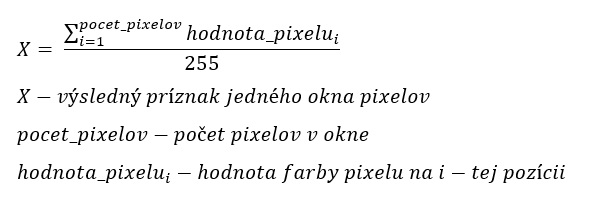
\includegraphics[width=10cm]{img/AddFeat.png}
  \caption{Výpočet príznaku okna pixelov}
  \label{MHIbox}
\end{figure}   

Takto vypočítané príznaky sme pridávali do vektoru príznakov na následné spracovanie a úpravu v PCA.

\subsubsection{Spracovanie pomocou PCA} \label{PCAim}
V algoritme \ref{PCAcreate} na extrakciu komponentov, ktorú sme si popísali v časti \ref{PCAlabel} sme použili metódy triedy \textit{\textbf{PCA}} knižnice \textit{sklearn}. Pre vytvorenie objektu PCA, sme použili parameter \textit{n\_components}, ktorý udáva počet komponentov, koľko chceme vybrať z vektora príznakov \textit{arrVectorFinal}. Tento počet komponentov musí byť nižší alebo nanajvýš rovný počtu vektorov príznakov. Natrénovaný model PCA s vektorom príznakov \textit{arrVectorFinal} sme uložili pre ďalšie spracovanie v SVM.

\begin{lstlisting}[
  caption={Trénovanie PCA},
  label={PCAcreate},
  language=python
]
pca = PCA(n_components)
pca.fit(arrVectorFinal)
joblib.dump(pca, 'ModelPCA.pkl')   
\end{lstlisting}

Trénovacia množina obsahuje 240 videí \textit{(6 tried po 40 videí)}, preto je aj maximálny počet hlavných komponentov, ktoré môžme získať z vektora príznakou pomocou PCA je 240. Teda výsledný vektor príznakov sa zmenšil na tie príznaky, ktoré sú najdôležitejšie. Neskôr v časti \ref{testalad} si ukážeme spôsoby, ktorými sme sa snažili naše výsledky ešte viac zlepšiť a vektor PCA rozšíriť.  


\subsection{Klasifikácia}
Pre natrénovanie klasifikátora sme sa rozhodli použiť SVM, ktorý sme popísali v časti \ref{SVMlabel}. Na implementovanie SVM sme použili triedu \textit{svm} z knižnice \textit{sklearn}. K dátam, ktoré máme uložené v \textit{arrVectorFinal} potrebujeme ešte označenie, ktorý vektor do akej kategórie patrí. Preto sme vytvorili ďalší vektor, v ktorom je pre každé video označenie kategórie, kam vektor patrí. Teraz už môžme natrénovať SVM. 
\hfill \break
\begin{lstlisting}[
  caption={Trénovanie klasifikátora},
  label={SVMcreate},
  language=python
]
clf = svm.SVC(decision_function_shape='ovr')
clf.fit(arrVectorFinal, classVector)
joblib.dump(clf, 'Model.pkl') 
\end{lstlisting}
Algoritmus \ref{SVMcreate} využíva volanie funkcií \textit{svm.SVC}, ktoré nám vytvorí klasifikátor \textit{(angl. Support Vector Classifier)}, rozhodovaciu funkciu sme zvolili \textit{ovr} \textit{(angl. one versus rest)}, keďže máme viac ako dve triedy pohybov. Následne prostredníctvom funkcie \textit{fit} sme natrénovali klasifikátor \textit{clf}, kde boli vložené vektory príznakov \textit{arrVectorFinal} a vektor tried \textit{classVector}. Takto natrénovaný model bolo potrebné uložiť pre ďalšie použitie a testovanie. 

\subsection{Priebežné testovania a ladenie} \label{testalad}
Po naprogramovaní všetkých základných častí nášho projektu sme potrebovali otestovať naše riešenie, či náš klasifikátor funguje dobre a či môžme prejsť ku finalizácii výsledkov, prípadne k ďalším vylepšeniam a zmenám.


\subsubsection{t-SNE}
Aby sme vedeli výsledok, ktorý ponúkajú nami vyextrahované príznaky, potrebovali sme výsledky vizualizovať, ako prebehlo rozdelenie do tried. Na to sme využili metódu založenú na redukcii dimenzií \textit{\acrfull{tsne}}, ktorej algoritmus nájdete v prílohe \ref{att:B}. V jazyku Python implementácia využíva na vizualizáciu dát knižnicu \textit{matplotlib}. Túto techniku je možné implementovať pomocou aproximácií, ktoré môžu byť aplikované na datasety obrovských rozmerov. Autorom tohto algoritmu je \textbf{\textit{Laurens van der Maaten}}, ktorý pôsobí ako výskumný pracovník na poli strojového učenia a počítačového videnia. t-SNE implementoval pre množstvo jazykov vrátane jazyka Python, takže sme nemali problém tento nástroj využívať. \cite{c18}



\subsubsection{Prvotné testy}
Ako prvý krok sme zvolili testovanie a tréning dvoch množín a teda beh a boxovanie. SVM sme natrénovali na tridsiatich videách z triedy behu a tridsiatich videách z triedy boxovania. 

Výsledok trénovania bol pre nás dobrý, keďže už vizuálne  na extrahovaných dátach bolo vidno rozdelenie týchto pohybov do dvoch tried. Výsledok je možné vidieť na obrázku \ref{Test2Class}. 

\begin{figure}[H]
  \centering
  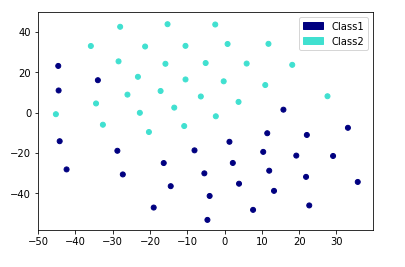
\includegraphics[width=14cm]{img/test2classes.png}
  \caption{Test dvoch tried pohybu}
  \label{Test2Class}
\end{figure} 


Ako príklad uvedieme taktiež pokus trénovania s jedným MHI, ktorý bol vytvorený vo 4. sekunde priebehu pohybu, avšak bez získania prídavných príznakov \ref{pridavny} a využitia metódy PCA.  Do tohto testu sme zapojili 5 tried pohybov, teda dataset KTH bez triedy pomalého behu, keďže sme usudzovali, že táto trieda sa dosť prelína medzi triedami behu a chôdze, čo sa ukáže aj na ďalších výsledkoch. 

Vyextrahované dáta, teda vektor príznakov a vektor tried sme znovu podrobili testu \textit{t-SNE}, kde výstup vyzeral ako na obrázku \ref{Test5Class1}, výsledky síce dávali zmysel, avšak rozdelenie jednotlivých tried nebolo až tak prehľadné ako sme si predstavovali. Triedy behu a chôdze pôsobia veľmi chaoticky, tak ako aj boxovanie s tlieskaním a zasahovaním kývania.

\begin{figure}[H]
  \centering
  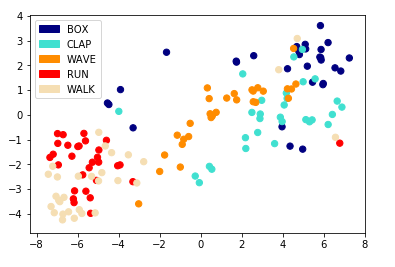
\includegraphics[width=14cm]{img/test5classes1.png}
  \caption{Prvý test piatich tried pohybu}
  \label{Test5Class1}
\end{figure}

Skúsili sme teda otestovať túto natrénovanú SVM, akú bude mať úspešnosť rozpoznávania. Výsledky môžte vidieť na obrázku \ref{Test5Class1g}.


\begin{figure}[H]
  \centering
  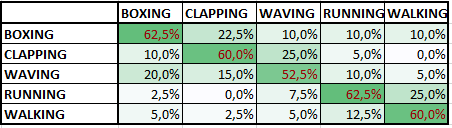
\includegraphics[width=14cm]{img/test5classes1tab.png}
  \caption{Úspešnosť 5 tried z 1 MHI}
  \label{Test5Class1g}
\end{figure}

Z tohto dôvodu sme sa rozhodli analyzovať náš postup a pristúpiť k optimalizácii riešenia, zbieraniu a ladeniu príznakov za pomoci viacnásobného využitia MHI, prídavných príznakov \ref{pridavny} a aplikovania PCA, ako bolo spomenuté v častiach \ref{HOGim}, \ref{PCAim}, \ref{pridavny}.


\subsubsection{Rozdelenie dát a finálne testy}
Dáta na tréning a testovanie sme rozdelili do dvoch skupín v pomere 40 testovacích videí a 40 trénovacích videí. Všetky testy boli vykonané na rovnakých videách, takže výsledky úspešnosti sú objektívne a porovnateľné pre každý typ konfigurácie programu.
Konfigurácie sme menili na 9 rôznych nastavení, pre ktoré sme natrénovali SVM a testovali ich úspešnosť pre všetky triedy pohybov databázy KTH viď obrázok \ref{tabTesty}.

\begin{figure}[H]
  \centering
  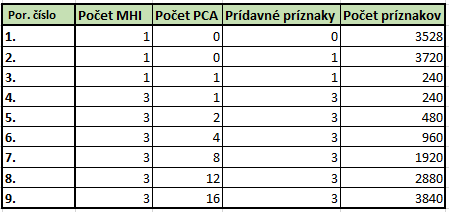
\includegraphics[width=14cm]{img/tabTesty.png}
  \caption{Konfigurácia trénovania a testovania}
  \label{tabTesty}
\end{figure} 

Ako vidno na obrázku, zvolili sme obmeny počtu MHI obrázkov s násobnými počtami vektorov pre získanie hlavných komponentov ako aj počet prídavných príznakov vypočítavaných z MHI. Stĺkec s názvom \textit{Počet MHI} udáva, koľko MHI obrázkov sme extrahovali z jedného videa, \textit{Počet PCA} udáva koľkonásobne rozšírený vektor sme spracovávali v PCA. \textit{Prídavné príznaky} označujú, z koľkých MHI obrázkov sme extrahovali dodatočné príznaky. \textit{Počet príznakov} určuje celkový počet extrahovaných príznakov na jedno video. 

\paragraph{1. Kofigurácia} 
V prvom teste s konfiguráciou jedného obrázku MHI, bez výpočtu PCA a prídavných príznakov sme dostali prvé výsledky \ref{test1}.

\begin{figure}[H]
  \centering
  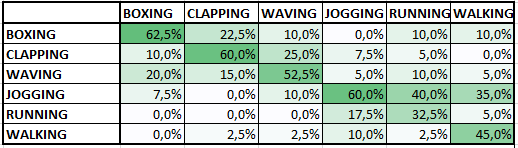
\includegraphics[width=14cm]{img/test6classes1g.png}
  \caption{Úspešnposť kofigurácie č. 1}
  \label{test1}
\end{figure} 

Z výsledkov je viditeľný problém medzi triedou \textit{Running} a \textit{Jogging}, kde zo všetkých testovaných videí behu vyhodnotilo až 40\% ako pomalý beh a 35\% chôdze vyhodnotilo ako pomalý beh. 


\paragraph{2. Kofigurácia} 
V druhom teste sme pridali ďalšie príznaky do vektora, výsledky pohybov sa zlepšili až na triedy behu, kde bol prepad až na úspešnosť 7,5\% a triedy behu, kde sa tiež znížila úspešnosť. Porovnanie je na obrázku \ref{test2}.


\begin{figure}[H]
  \centering
  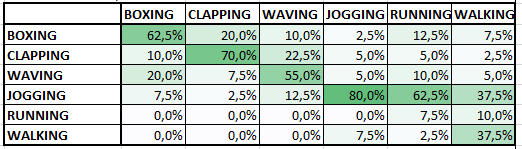
\includegraphics[width=14cm]{img/test6classes11g.png}
  \caption{Úspešnposť kofigurácie č. 2}
  \label{test2}
\end{figure} 

\paragraph{3. Kofigurácia} 
V tomto teste sme sa rozhodli zistiť vplyv PCA na celkové riešenie problému. Výsledky ukázali všeobecné zlepšenie, hlavne v triede mávania rukami, kde sa úspešnosť zvýšila z 55\% na 72.5\%.  
\begin{figure}[H]
  \centering
  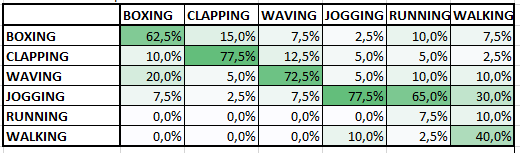
\includegraphics[width=14cm]{img/test6classes11PCA1g.png}
  \caption{Úspešnposť kofigurácie č. 3}
  \label{test3}
\end{figure} 


\paragraph{4. Kofigurácia} 
V nasledujúcich testoch nás zaujímal vplyv trojnásobného použitia obrázkov MHI na výsledky a úspešnosť testovania v spolupráci s rozširovaním PCA. Použili sme MHI z prvých 4, 6 a 9 sekúnd videa. Objavilo sa nepatrné zlepšenie až na prepad úspešnosti triedy \textit{Jogging}, v ktorom úspešnoť od predchádzajúceho testu klesla o 17,5\%. Finálny počet príznakov na jeden vektor bol 240.

\begin{figure}[H]
  \centering
  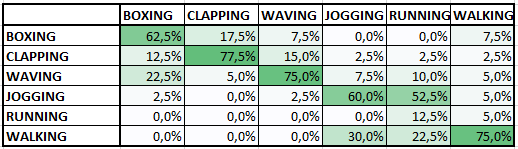
\includegraphics[width=14cm]{img/test6PCA1g.png}
  \caption{Úspešnposť kofiguráciet č. 4}
  \label{test4}
\end{figure} 

\paragraph{5. Kofigurácia} 
V nasledujúcom teste sme iba zdvojnásobili počet vektorov príznakov videí (480 príznakov na video), aby sme mohli pomocou PCA vypočítať dvojnásobný počet príznakov ako v predchádzajúcom teste. Z výsledkov nám vyplynulo, že tento postup rozširovania počtu vektorov sa nám môže vyplatiť, keďže sa nám výsledky nezhoršili a v triede \textit{Waving} sme dokonca dostalo výsledok lepší o 2,5\%. 
\begin{figure}[H]
  \centering
  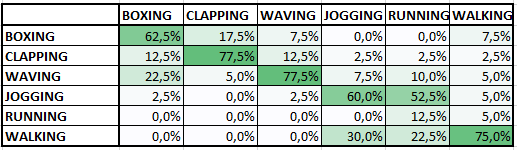
\includegraphics[width=14cm]{img/test6PCA2g.png}
  \caption{Úspešnposť kofigurácie č. 5}
  \label{test5}
\end{figure} 

\paragraph{6. Kofigurácia} 
Test so štvornásobne zvýšeným počtom vektorov (960 príznakov na video) nám znovu priniesol zlepšenie v triede \textit{Waving} a to dokonca o celých 5\%. Vzhľadom na to, že sa nám výsledky stále zlepšovali, snažili sme sa ísť ešte ďalej.
\begin{figure}[H]
  \centering
  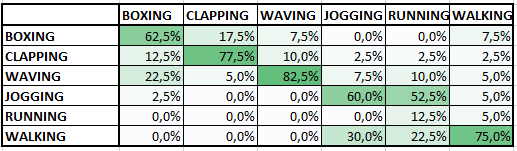
\includegraphics[width=14cm]{img/test6PCA4g.png}
  \caption{Úspešnposť kofigurácie č. 6}
  \label{test6}
\end{figure} 

\paragraph{7. Kofigurácia} 
Siedmy test s osemnásobným zväčšením počtu vektorov (1920 príznakov na video) nám znovu vylepšil výsledky o 2,5\% pre triedy \textit{Clapping} a \textit{Waving}. Stále to nemalo žiaden negatívny vplyv na ostatné výsledky.
\begin{figure}[H]
  \centering
  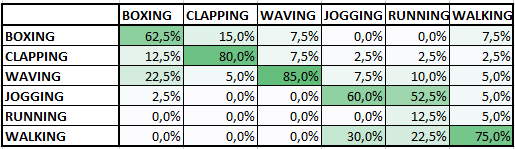
\includegraphics[width=14cm]{img/test6PCA8g.png}
  \caption{Úspešnposť kofigurácie č. 7}
  \label{test7}
\end{figure} 

\paragraph{8. Kofigurácia}
Pri teste, kde sme zvolili 12-násobné rozšírenie (2880 príznakov na video) počtu vektorov sa nám už zlepšovanie výsledkov zastavilo. Pri testoch sme namerali identické hodnoty, čo nám naznačovalo, že ďalšie zvyšovanie počtu vektorov nám už nebude naše výsledky vylepšovať. Týmto by sme mohli konfiguráciu, ktorá bola nastavená v tomto teste, respektíve v teste predchádzajúcom, považovať za najvhodnejšie zvolenú a porovnať ju s inými riešeniami.
\begin{figure}[H]
  \centering
  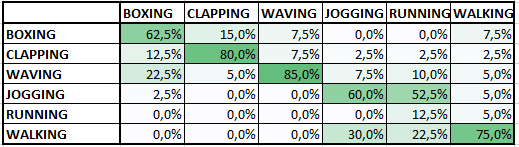
\includegraphics[width=14cm]{img/test6PCA12g.png}
  \caption{Úspešnposť kofigurácie č. 8}
  \label{test8}
\end{figure}  

\paragraph{9. Kofigurácia} 
Ako sme sa predpokladali, výsledky pri 16-násobnom rozšírení (3840 príznakov na video) sa vôbec nezlepšili, naopak, v triede \textit{Jogging} sme zaznamenali pokles o 2,5\% z úspešnosti. 
\begin{figure}[H]
  \centering
  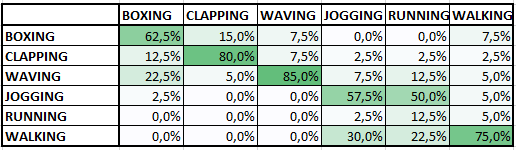
\includegraphics[width=14cm]{img/test6PCA16g.png}
  \caption{Úspešnposť kofigurácie č. 9}
  \label{test9}
\end{figure} 

Pri tomto výsledku môžme konštatovať, že výsledky sú uspokojujúce až na veľmi nízku úspešnosť triedy \textit{Running}, ktorá sa až na 52,5\% obmieňa s triedou \textit{Jogging} a na 22,5\% s triedou \textit{Walking}. Pre naše riešenie to nepovažujeme za veľký problém vzhľadom na to, že pohyby v ktorých sa náš algoritmus mýlil a zamieňal si ich, sú veľmi podobné, rozdiel je iba v rýchlosti jednotlivých aktérov na videu, kde niektorí pri pomalom behu pomaly kráčali a naopak. 




\section{Porovnanie s existujúcim riešením}
Pre porovnanie nášho riešenia sme si vybrali prácu, v ktorej pracovali s tou istou databázou videí ako my v našej práci. V porovnávanom riešení využívajú lokálne časovo-priestorové príznaky. Tieto pohybové príznaky následne trénujú pomocou SVM. 

Na testovanie úspešnosti SVM využili viacero scenárov:

\begin{itemize}
\item \textbf{S1 - vonkajšie prostredie}
\item \textbf{S2 - vonkajšie prostredie s variabilnou vzdialenosťou}
\item \textbf{S3 - vonkajšie s rôznym oblečením}
\item \textbf{S4 - vo vnútri}
\end{itemize}

\subsection{Výsledky}
V práci majú reprezentované dva výsledky. Priemer výsledkov pre všetky štyri scenáre a pre scenár S2.

\subsubsection{Všetky scenáre}

Na obrázku \ref{cmp1} sú spriemerované výsledky všetkých scenárov. 
\begin{figure}[H]
  \centering
  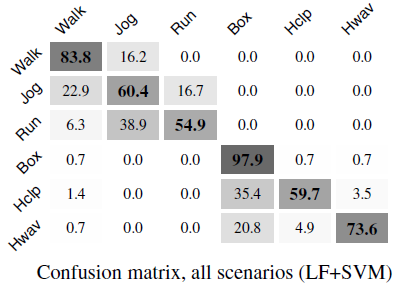
\includegraphics[width=10cm]{img/cmpLFSVM.png}
  \caption{Výsledky všetkých scenárov}
  \label{cmp1}
\end{figure}  

Z výsledkov môžme usúdiť, že všetky kategórie im zaradilo s viac ako 50\%-tnou úspešnosťou. 
Oproti nášmu riešeniu sa im podarilo lepšie vyhodnotiť pohyb behu o 42,4\%,  boxu o 35.4\%, chôdze o 8,8\% a pomalý beh o zanedbateľných 0.4\%.

Naopak zhoršenie oproti nášmu výsledku sme zaznamenali pri pohybe potlesku - o 20,3\% a kývaniu oboma rukami o 11,4\%.

Tieto výsledky pôsobia celkom slušne, vzhľadom na to, že neobsahujú vysokú chybu pri pohybe behu ako v našom riešení.


\subsubsection{Scenár S2}
V tomto teste testovali na jednom scenári vo vonkajšom prostredí. Výsledky sú na obrázku \ref{cmp2}. 

\begin{figure}[H]
  \centering
  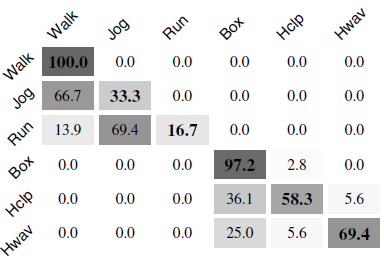
\includegraphics[width=10cm]{img/cmpLFSVM2.png}
  \caption{Výsledky scenára S2}
  \label{cmp2}
\end{figure}  

V týchto výsledkoch môžme skonštatovať, že naše výsledky boli nižšie v pohyboch boxu o 34,7\%, pohybe behu o 4,2\% a pohybe chôdze o 25\%, kde sa im podarilo správne rozpoznať všetky testovacie videá.

Na opačnej strane v našich výsledkoch sa nám viac darilo pri pochyboch tlieskania o 21,7\%, pohybe kývania o 15,6\%, pohybe pomalého behu o 26,7\%. 

V oboch prípadoch sme zaznamenali vysoký podiel zamieňania pohybu behu s pomalým behom, respektíve chôdzou. Taktiež vysoké percento pomalého behu bolo zaregistrované ako chôdza či v našom, alebo ich riešení. 

Zamieňanie týchto pohybov si môžme odôvodniť ich podobnosťou, keďže každá osoba beží, respektíve chodí inou rýchlosťou. To, čo je u niekoho pomalým behom je pre iného chôdzou. Týmito argumentami si zastávajú názor aj v porovnávanom riešení. 

\subsubsection{Zhodnotenie výsledkov}
Výsledky, ktoré sme dosiahli sú uspokojivé, vzhľadom na metódy, ktoré sme použili môžme prehlásiť, že sa nám podarilo vytvoriť klasifikátor, ktorý dokáže rozpoznať jednotlivé typy pohybov na základe ich časovo-priestorových vzťahov.

Vidíme aj priestor na vylepšenie riešenia, ktoré by mohlo byť predmetom ďalšieho skúmania. 


 









